%------------------------------------------------------------------------------
% Template file for the submission of papers to IUCr journals in LaTeX2e
% using the iucr document class
% Copyright 1999-2013 International Union of Crystallography
% Version 1.6 (28 March 2013)
%------------------------------------------------------------------------------

%xxxxxx just for testing github % 2
%xxxxxx just for testing github % 3

\documentclass[preprint]{iucr}              % DO NOT DELETE THIS LINE
%\documentclass[]{iucr}              % DO NOT DELETE THIS LINE
\usepackage{amssymb}
\usepackage[fleqn]{amsmath}
%\usepackage{xtabular]
%\usepackage{bm}
\usepackage{longtable}
\usepackage{graphicx}
\usepackage{tabularx}
\usepackage{booktabs}
%\usepackage{calligra}
\usepackage{array}
 \usepackage{setspace}
 \DeclareMathAlphabet{\mathcalligra}{T1}{calligra}{m}{n}
\def\mathbi#1{\textbf{\em #1}}
\numberwithin{equation}{section}
%\DeclareMathSymbol{\Gamma}{\mathalpha}{letters}{"00}
%\DeclareMathSymbol{\Lambda}{\mathalpha}{letters}{"03}
%\DeclareMathSymbol{\Omega}{\mathalpha}{letters}{"0A}
%\DeclareMathAlphabet{\mathitbf}{OML}{cmm}{b}{it}
\hyphenation{Niggli}
\def\mathbi#1{\textbf{\em #1}}
%\numberwithin{equation}{section}
%\DeclareMathSymbol{\Gamma}{\mathalpha}{letters}{"00}
%\DeclareMathSymbol{\Lambda}{\mathalpha}{letters}{"03}
%\DeclareMathSymbol{\Omega}{\mathalpha}{letters}{"0A}
%\DeclareMathAlphabet{\mathitbf}{OML}{cmm}{b}{it}
\usepackage{color}
\usepackage{ulem}
\usepackage{url}
\usepackage{yfonts}
%\usepackage{xr-hyper}
%\usepackage[draft]{hyperref}
%\usepackage{bibentry}
\newcommand{\BIV}[0]{$\bf{B^{4}}$}
\newcommand{\SVI}[0]{$\bf{S^{6}}$}
\newcommand{\GVI}[0]{$\bf{G^{6}}$}
\newcommand{\CIII}[0]{$\bf{C^{3}}$}
\newcommand{\DVII}[0]{$\bf{D^{7}}$}
\newcommand{\DXIII}[0]{$\bf{DC^{13}}$}
\newcommand{\VVII}[0]{$\bf{V^{7}}$}

\newcommand{\vdotv}[2]{${{\bf #1 \cdot #2}}$}
\newcommand{\Imaginary}[0]{$ \textfrak{I} $}
\newcommand{\Real}[0]{$ \textfrak{R} $}
\newcommand{\Exchange}[0]{$\textfrak{X}$}

\newcommand{\nounderline}[3]{\!\!\!\!\!\!\!\!\!#1,&\!\!\!\!\!\!\!\!\!#2,&\!\!\!\!\!\!\!\!\!#3}
\newcommand{\underlineab}[3]{\!\!\!\!\!\!\!\!\!\!\!\!\!\!\!\!\!\!\!\!\!\!\!\!\Exchange{}(#1),&\!\!\!\!\!\!\!\!\!\!\!\!\!\!\!\!\!\!\!\!\!\!\!\!\Exchange{}(#2),&\!\!\!\!\!\!\!\!\!#3}
\newcommand{\underlineac}[3]{\!\!\!\!\!\!\!\!\!\!\!\!\!\!\!\!\!\!\!\!\!\!\!\!\Exchange{}(#1),&\!\!\!\!\!\!\!\!\!\!\!\!\!\!\!\!\!\!\!\!\!\!\!\!#2,&\!\!\!\!\!\!\!\!\!\Exchange{}(#3)}
\newcommand{\underlinebc}[3]{\!\!\!\!\!\!\!\!\!\!\!\!\!\!\!\!\!\!\!\!\!\!\!\!#1,&\!\!\!\!\!\!\!\!\!\Exchange{}(#2),&\!\!\!\!\!\!\!\!\!\!\!\!\!\!\!\!\!\!\!\!\!\!\!\!\Exchange{}(#3)}

\newcommand{\scalar}[1]{$#1$}

\newcommand{\scalarsub}[2]{$#1_#2$}


%-------------------------------------------------------------------------
% Information about journal to which submitted
%-------------------------------------------------------------------------
%\journalcode{A}              % Indicate the journal to which submitted
%   A - Acta Crystallographica Section A
%   B - Acta Crystallographica Section B
%   C - Acta Crystallographica Section C
%   D - Acta Crystallographica Section D
%   E - Acta Crystallographica Section E
%   F - Acta Crystallographica Section F
%   J - Journal of Applied Crystallography
%   M - IUCrJ
%   S - Journal of Synchrotron Radiation
\makeatletter
\font\dummyft@=dummy \relax
\makeatother

\DeclareMathOperator{\mr}{\textfrak{P}_i}
\begin{document}                  % DO NOT DELETE THIS LINE
	\singlespacing

	
	%-------------------------------------------------------------------------
	% The introductory (header) part of the paper
	%-------------------------------------------------------------------------
	
	% The title of the paper. Use \shorttitle to indicate an abbreviated title
	% for use in running heads (you will need to uncomment it).
	
	% Authors' names and addresses. Use \cauthor for the main (contact) author.
	% Use \author for all other authors. Use \aff for authors' affiliations.
	% Use lower-case letters in square brackets to link authors to their
	% affiliations; if there is only one affiliation address, remove the [a].
	
	% Use \vita if required to give biographical details (for authors of
	% invited review papers only). Uncomment it.
	
	% lca IUCr id IUCr6401
	%\vita{Author's biography}
	
	% Keywords (required for Journal of Synchrotron Radiation only)
	% Use the \keyword macro for each word or phrase, e.g. 
	% \keyword{X-ray diffraction}\keyword{muscle}
	
	
	% PDB and NDB reference codes for structures referenced in the article and
	% deposited with the Protein Data Bank and Nucleic Acids Database (Acta
	% Crystallographica Section D). Repeat for each separate structure e.g
	% \PDBref[dethiobiotin synthetase]{1byi} \NDBref[d(G$_4$CGC$_4$)]{ad0002}
	
	%\PDBref[optional name]{refcode}
	%\NDBref[optional name]{refcode}
	
	%-------------------------------------------------------------------------
	% The introductory (header) part of the paper
	%-------------------------------------------------------------------------
	
	% The title of the paper. Use \shorttitle to indicate an abbreviated title
	% for use in running heads (you will need to uncomment it).
	{\Large PDF generated: \emph{\today}} \\
	\title{Command line programs from LatticeRepLib}
	\shorttitle{Command line programs}
	
	% Authors' names and addresses. Use \cauthor for the main (contact) author.
	% Use \author for all other authors. Use \aff for authors' affiliations.
	% Use lower-case letters in square brackets to link authors to their
	% affiliations; if there is only one affiliation address, remove the [a].
	
	
	\cauthor[a]{Lawrence C.}{Andrews}{lawrence.andrews@ronininstitute.org}{}
	\author[b]{Herbert J.}{Bernstein}
	
	\aff[a]{Ronin Institute, 9515 NE 137th St, Kirkland, WA, 98034-1820 \country{USA}}
	\aff[b]{Ronin Institute, c/o NSLS-II, Brookhaven National Laboratory, Upton, NY, 11973 \country{USA}}
	
	% Use \shortauthor to indicate an abbreviated author list for use in
	% running heads (you will need to uncomment it).
	
	\shortauthor{Andrews and Bernstein}
	
	% Use \vita if required to give biographical details (for authors of
	% invited review papers only). Uncomment it.
	
	% lca IUCr id IUCr6401
	%\vita{Author's biography}
	
	% Keywords (required for Journal of Synchrotron Radiation only)
	% Use the \keyword macro for each word or phrase, e.g. 
	% \keyword{X-ray diffraction}\keyword{muscle}
	
	%	\keyword{Delaunay}
	%	\keyword{Delone}
	%	\keyword{Selling}
	%	\keyword{\CIII}
	
	% PDB and NDB reference codes for structures referenced in the article and
	% deposited with the Protein Data Bank and Nucleic Acids Database (Acta
	% Crystallographica Section D). Repeat for each separate structure e.g
	% \PDBref[dethiobiotin synthetase]{1byi} \NDBref[d(G$_4$CGC$_4$)]{ad0002}
	
	%\PDBref[optional name]{refcode}
	%\NDBref[optional name]{refcode}
	\maketitle                        % DO NOT DELETE THIS LINE
	
	\begin{synopsis}
		Selling reduction and Delone reduction are
		considered in a space of complex variables.
	\end{synopsis}
	\newcommand{\si}[0]{$s_1$}
	\newcommand{\sii}[0]{$s_2$}
	\newcommand{\siii}[0]{$s_3$}
	\newcommand{\siv}[0]{$s_4$}
	\newcommand{\sv}[0]{$s_5$}
	\newcommand{\svi}[0]{$s_6$}
	\newcommand{\Svec} [0] {\{\si, \sii, \siii, \siv, \sv, \svi \}}
	\newcommand{\SvecA} [0] {\{-\si, -\si+\sii, \si+\siii, \si+\sv, \si+\siv, \si+\svi \}}
	
	\newcommand{\OPES}[0]{$E^3toS^6$}
	\newcommand{\OPESS}[0]{$$E^3toS^6$$}
	\newcommand{\MSVI}[0]{$M_{S^{6}}$}
	\newcommand{\MEIII}[0]{$M_{E^{3}}$}
	\newcommand{\Plus}[0]{$\textfrak{P}$}	
	\newcommand{\Minus}[0]{$\textfrak{M}$}
	
	\newcommand{\ci}[0]{$c_1$}
	\newcommand{\cii}[0]{$c_2$}
	\newcommand{\ciii}[0]{$c_3$}
%	\begin{abstract}
%	\end{abstract}
	
	
	\section{Introduction}
	
	
	In the study of various spaces for representing lattices, a
	number of software tools have been prepared. Some of those
	are available as simple commandline programs. Most of them
	have flexible input and output their processed results in 
	a form that another can use that for processing. A few
	are terminal programs that produce analysis. A small
	number take no input and generate files for other uses.
	
	
	
	% Appendices appear after the main body of the text. They are prefixed by
	% a single \appendix declaration, and are then structured just like the
	% body text.
	
	\section{Data Inputs:}
	\subsection{Table of input types}
	
	In general, there are 5 types of input lines, see Table \ref{inputtypes}.
	Except for "END", they can be combined in any order.
	
	\begin{table}
		\label{inputtypes}
		\caption{	All these are case-insensitive. If a particular
			input lattice is invalid, it is rejected with a message.}
		\begin{tabular}{l p{.2\textwidth} l l l}
			\toprule
			
			\begin{tabular}{l l l l}
				\underline{\textbf{Vector Input:}}&
				\parbox[t]{0.6\textwidth}{\textbf{g} 
					 for \GVI{} vectors\\
					\textbf{s} for \SVI{}, Delone/Selling scalars\\
					\textbf{C3} for \CIII{} input (without parentheses or commas, \\
					~~~“C” would be interpreted as a C-centered unit cell)\\
					\textbf{U} for DC7 unsorted}\\
			\end{tabular}	\\[3pt]
			
			\underline{\textbf{RANDOM:}} Random (valid) unit cell generated\\
			
			\underline{\textbf{Crystal lattice input:}} 
			``\textbf{A}'', ``\textbf{B}'', ``\textbf{C}'', ``\textbf{P}'', ``\textbf{R}'', ``\textbf{H}'',``\textbf{F}'', ``\textbf{I}''	\\
			~~~~~followed by three axis lengths and three angles (in degrees)\\
			\underline{\textbf{semicolon}}: 
			lines beginning with a semicolon are treated as comments\\
			\underline{\textbf{END:}} ends the data input section\\
			\bottomrule
		\end{tabular}
		
	\end{table}	
	\subsection{Examples of unit cell inputs}
	\noindent
	P 10 20 30 90 111 90\\
	G 100 400 900  0 -215.02 0\\
	S6   0 -107.51  0   7.51 -400 -792.49\\
	; this is a comment
	
	\section{Programs}
	
	\subsection{Filters - change lattice representation}
	
	\begin{table}
		\renewcommand{\arraystretch}{1.2}
		\caption{Programs to convert lattice representations.
		NOTE: although all can take all of the input types, \BIV{}. \DXIII{}, 
	Polar write output that cannot be used as input.}
		\begin{tabular}{l l l p{.7\textwidth}  l}
			\toprule
			Name		&	in	&	out			& Output	\\
			\midrule
			CmdToB4		&	y	&	\BIV{}		&		For each input, 
			it produces the 4 vectors as a,b,c,d as E3 vectors, 
			and also the lengths of each of those vectors.\\[.9pt]
			CmdToC	3	&	y	&	\CIII{	}	&		
			For each input, produces the \CIII{} representation in the form 
			(\#,\#) (\#,\#) (\#,\#), 
			which does not conform to the format for input to other programs.\\[.9pt]
			CmdToCell	&	y	&	
			\parbox[t]{0.07\textwidth}{${	a,b,c,}$ \\ ${\alpha,\beta,\gamma}$}	&					Converts to the conventional unit cell representation
			If the input is already unit cell parameters, then the output
			will be in the same lattice centering as the input.\\[.9pt]
			CmdToDC		&	y	&	\DXIII{}		&	Outputs the lengths of the 13 unique vectors describing the Dirichlet cell.\\[.9pt]			
			CmdToG6		&	y	&	\GVI{}		&		Converts the input to \GVI{}\\[.9pt]
			CmdToS6		&	y	&	\SVI{}		&		Converts the input to \SVI{}\\[.9pt]
			Radial		&	y	&	Polar	&
				CSomputes the polar distances in Angstroms 
				from the first input cell. 
				That is {(a,$\alpha$)}, {(b,$\beta$)}, and {(c,$\gamma$)} 
				as coordinates in complex space.\\[.9pt]
			\bottomrule
			
		\end{tabular}
	\end{table}

\subsection{Data processing programs}

		\begin{longtable}{l l l p{.2\textwidth} p{.5\textwidth} l}
			\caption{Summary of programs manipulating data}
			\label{processingprogs}\\ %NOTE: that lineskip is necessary to prevent toprule from crashing
			\toprule
			Name		&	in	&	out		&	\begin{parbox}[t]{2cm}{
				command line\\
				param{s}}
			\end{parbox}	& Output	\\[.9pt]
			\midrule
			CmdCmplx	&	NA	&	y		&\hrulefill	&Currently, 
				this just outputs some programmed examples.		\\[.9pt]
			CmdDelone	&	y	&	\SVI{}	&\hrulefill	&Converts input to \SVI{}		\\[.9pt]
			CmdDists	&	y	& mod		&\hrulefill	&For on input list of n
			cells, n-1 distances will be output.\\[.9pt]
			CmdGen		&	NA	&	\GVI{}	&	ngen	&- number of examples to generate (optional)\\
				{}		&		&			&type		& - lattice type to 
				generate (optional); many options 
				c,t,h,o,r,h,m,a, 
				cP, cF,cI, tP, tI, hP, hR, oP, oF, oI, oS, mP, mC, mS, aP, 
				numeric Niggli types - 1-44, 
				Delone types - C1,C3,C5,~\dots 
				If no parameters are present, one each of the 44 Niggli types. 
				If only a number is present, that is how many of each of the 44 Niggli types to generate.
				For usage examples, see Table \ref{CMDGENexamples}\\[.9pt]
			CmdLM		&	y	&	y		&	\hrulefill		&		Lattice Matching. 
				The first input cell is used as the reference. 
				Succeeding cells are matched 
				as well as possible to the reference cell.\\[.9pt]
			CmdNiggli	&	y	&	\GVI{}	&\hrulefill	&		
				Produces the Niggli reduced cell for 	each input.\\[.9pt]
			CmdPath		&	y	& \SVI{}			&
			no. of points	& If the number of points is 
			not on the command line, the default number 
			to generate is 20.	If there is only one point, 
			then the second point is generated as the 
			Niggli reduced cell. If more than two points are input, 
			each successive pair will
			generate a list of output points; so if
			3 cells are input, the output will be 
			2 times the number of points requested.	\\[.9pt]
			CmdPerturb	&	y	& y			&	n-number of perturbations, 
			
				parts per thousand to perturb			&
				n cells perturbed normal to the input \SVI{} vector
				If a lattice centering (including P) is input,
				the output is in the same centering. Otherwise, the output is in \SVI{}.	\\[.9pt]
			CmdS6Refl	&	y	&	\SVI{}	&\hrulefill	&	For each input, 
				all 24 \SVI{} reflections are produced.\\[.9pt]
			CmdSella	&	y	&	y		&\hrulefill	&
				SELLA produces 2 output: std::out contains the match of
				each of the 24 Delone types; SVG for the Grimmer
				diagram is written to a file with a name such as 
					\verb#SEL__2023-01-07.08_56_42.svg# with date/time stamp.\\
			CmdSort		&	y	&	y		&"C3" or "seq'&	CmdSort has 2 possible actions. If "seq" is specified
			as the sort type, then in the incoming list of 
			lattices, in each pair, the second one is multipled by the 24 \SVI{} reflections, and the one that
			is closest to the first is chosen for output.\\[.9pt]
			CmdVolume	&	y	&	mod		&\hrulefill	&		Outputs the unit cell 
				and the volume of each input cell.\\[.9pt]
%			MultiMetricDists&y	& mod		&"Y/y"(optional)&	
%				Parameter Y/y for maxima style output		\\[.9pt]
			PlotC3		&	y	&	mod		& \hrulefill	& Plot 
				the three \CIII{} coordinates. See Figure~\ref{plotc3}. The gray lines
				connect successive pairs of points 
				in the input. The output graphics file
				is an SVG file whose name is in the output
				in standard output.\\[.9pt]
			SELLA		&	y	&	mod		&\hrulefill	&	
				Outputs the distances from each of the Bravais lattice types 
				(in \svi{}).	\\[.9pt]
			SVD			&	y	&	mod		&\hrulefill	& Outputs the singular value decomposition vectors
				and eigenvalues for the input lattice. This is done in \SVI{}.		\\[.9pt]			
			\bottomrule
			
		\end{longtable}
%	\end{table}
	
	\begin{itemize}
		  \setlength\itemsep{3em}
	\item{\textbf{CmdGen}}
	
	\subsection{Individual program details}

CmdGen is a program for creating examples of various types of lattice types.
		
There are two optional input parameters. The first is the count
of how many samples of each type to generate. The second (if present) is
the type of lattices to generate.  There is no input data
other than the command line parameters.

For examples of using CmdGen, see table \ref{CMDGENexamples}


The is considerable flexibility in the input types. However, they
are case-sensitive.


\begin{itemize}
	\item Niggli types by number 1-44 (see Table \ref{NiggliFormsI}).
\begin{singlespace}
		\item Delone types by Delone's designation - 
	C1,C3,C5, T1, T2, T5, R1, R3,\\ 
	O1A, O2, O3, O4, O5, O1B, M1A, M2A, M3, M4, M1B, M2B, 
	A1, A2, A3, H4 (see Table \ref{s6table}).
\end{singlespace}
	\item Crystal system - c,h,t,o,m,a
\end{itemize}


\vspace{2pt}

\begin{table}
		
		\label{CMDGENexamples}
		\caption{CmdGen examples}

		
		\begin{tabular}{l l l l}
			\midrule
			CmdGen & generates a single example of each of the 44 Niggli types\\[2pt]
			CmdGen 2 & generates two examples of each of the 44 Niggli types\\[2pt]
			CmdGen 4 aP & generates four examples of each of the two anorthic Niggli types\\[2pt]
			CmdGen 2 17& generates 2 examples of Niggli 17, which is mC\\
			{}&\textbf{Output}:\\
			{}&; Niggli lattice type requested\\
			{}&; lattice type = 17\\
			{}&G6    90.428    90.428   142.222    83.992    83.992    22.888   IT\# = 17  mC\\
			{}&G6    79.033    79.033   111.127   -61.421   -73.872   -22.772   IT\# = 17  mC\\
			CmdGen 2 C5& generate two examples of Delone type "C5", which is
			primitive cubic.\\
			{}&\textbf{Output}:\\
			{}&; Delone lattice type input\\
			{}&; lattice type = C5\\
			{}&G6   181.275   181.275   181.275     0.000     0.000     0.000   IT\# = C5  cP\\
			{}&G6    74.526    74.526    74.526     0.000     0.000     0.000   IT\# = C5  cP\\[2pt]
			
			CmdGen 1 h& Generate a single example of each of the hexagonal (and rhombohedral) Bravais lattice (per Niggli).\\
			{}&\textbf{Output}:\\
			{}&; Niggli lattice type input\\
			{}&; lattice type = 2\\
			{}&G6   119.828   119.828   119.828   -45.302   -45.302   -45.302   IT\# = 2  hR\\
			{}&;\\
			{}&; lattice type = 4\\
			{}&G6    86.837    86.837    86.837    19.813    19.813    19.813   IT\# = 4  hR\\
			{}&;\\
			{}&; lattice type = 9\\
			{}&G6     3.688     3.688   145.128     3.688     3.688     3.688   IT\# = 9  hR\\
			{}&;\\
			{}&; lattice type = 12\\
			{}&G6    55.273    55.273   136.854     0.000     0.000   -55.273   IT\# = 12  hP\\
			{}&;\\
			{}&; lattice type = 22\\
			{}&G6    73.578    73.578   149.339     0.000     0.000   -73.578   IT\# = 22  hP\\
			{}&;\\
			{}&; lattice type = 24\\
			{}&G6   101.390   125.771   125.771   -91.974   -67.593   -67.593   IT\# = 24  hR\\
			{}&;\\
			\bottomrule
		\end{tabular}	
	\end{table}	
	
	
	\item \textbf{SVD}
	
	On input to a number of lattices, 
	SVD calculates a Singular Value Decomposition.
	The output consists of the eigenvalues and 
	the six eigenvectors.
	It is important to check that the form of
	each cell is the same; for instance, monoclinic
	cell should have the unique interaxial angle
	in the same place (\textit{e.g.} $\beta$)\\
	
	As an example, consider using SVD to compute the information
	for one of the 
	
	\begin{samepage}
		{\nopagebreak{
				\textbf{Command line:}\\
				CmdGen 5 33 \textbar~ CmdSort seq \textbar~ SVD\\
				; SVD\\
				S6 from input cell   0.000 -31.196   0.000 -71.963 -109.653 -131.880\\
				S6 from input cell   0.000 -23.060   0.000 -77.367 -110.398 -125.599\\
				S6 from input cell   0.000 -28.898   0.000 -54.985 -106.336 -82.229\\
				S6 from input cell   0.000 -56.133   0.000 -103.736 -177.343 -123.204\\
				S6 from input cell   0.000 -10.111   0.000 -50.618 -91.57100 -98.102\\
			}
		}
	\end{samepage}
	
	\begin{samepage}
		\nopagebreak{
			\textbf{Output}:\\
			\textbf{eigenvalue     0};         vector         1 0 0 0 0 0\\
			eigenvalue 413.012;       vector         0 -0.1728 00 -0.4007 -0.6616 -0.6097\\
			eigenvalue 48.3869;       vector         0 -0.4009 0 -0.1129 -0.5164 0.7482\\
			eigenvalue 14.0785;       vector         0 -0.7060 0 -0.4581 0.5344 -0.0786\\
			eigenvalue 8.53435;       vector         0 0.5576 0 -0.7853 0.1001 0.2494\\
			\textbf{eigenvalue     0};         vector         0 0 -1 0 0 0
		}
	\end{samepage}
	
	The two zero eigenvalues correspond to the invariant
	interaxial angles ($\alpha$ and $\gamma$, in this case).
	
	\item \textbf{CmdS6Refl}
	
	CmdS6Refl generates the 24 reflections (see \cite{Andrews2019b})
	of each input lattice. Duplicate outputs of each input are not removed.
	
		
	\item \textbf{CmdPath}
	
	CmdPath outputs points along a line between pairs of lattice.
	
	The number of points per segment is a commandline parameter.
	If no parameter is input, the default is 20. This is not
	the number of steps; it is the number of points that will be
	output for a segment (pair of input lattices).
	
\begin{enumerate}
	\item Only a single lattice is input. A second point will
	be generated as the Niggli reduced lattice, and series of points
	will be output between them.
	
	\item Two lattices are input. Then the points will be
	created between them.
	
	\item More than two lattices are input. Then each point
	and its succeeding point will generate a segment. Each segment
	will be output as the number of points specified. Note: the
	final point of one segment and the first point of the next
	segment will be duplicates.
\end{enumerate}
	
	The line between points is calculated in \SVI{}. The other
	likely space would be \GVI{}, but the results seem to be the same.
	As an example, in the case of 3 items input and 5 requested
	output lattices, the output will consist of 10 lines, 5
	for each successive pair of lattices, and the 5th and
	6th points will be the same.\\
	
	\textbf{Command Line:}\\
	 CmdPath 5 \\
	; Path generator\\
	f 10 10 10 90 90 90 90\\
	end\\
	
	\textbf{Output:}\\
	; no. of points output is 5\\
	S    0.00000   0.00000   0.00000 -100.00000 -100.00000 -100.00000    1\\
	S    6.25000   6.25000   6.25000 -100.00000 -100.00000 -100.00000    2\\
	S   12.50000  12.50000  12.50000 -100.00000 -100.00000 -100.00000    3\\
	S   18.75000  18.75000  18.75000 -100.00000 -100.00000 -100.00000    4\\
	S   25.00000  25.00000  25.00000 -100.00000 -100.00000 -100.00000    5\\
	
	\textbf{Command Line:}\\
	 CmdPath 5  \textbar~ CmdToCell\\
	; To Cell\\
	f 10 10 10  90 90 90\\
	end\\
	
	\textbf{Output:}\\
	; no. of points output is 5\\
	P  10.00000  10.00000  10.00000  90.00000  90.00000  90.00000\\
	P   9.35414   9.35414   9.35414  85.90396  85.90396  85.90396\\
	P   8.66025   8.66025   8.66025  80.40593  80.40593  80.40593\\
	P   7.90569   7.90569   7.90569  72.54240  72.54240  72.54240\\
	P   7.07107   7.07107   7.07107  60.00000  60.00000  60.00000\\
	
	
\end{itemize}

	
		\begin{table}
		\caption{The table of \citeasnoun{Delaunay1932} describing the 24
			Bravais types in \SVI{}. It has been redone removing the images of the 
			Dirichlet cells, the not-reduced cells, and adding the ''lattice character", which
			describes the linear manifold of each type. The crystal family types have been
			renamed to modern usage: Q changed to T for tetrahedral, K changed
			to C for cubic, and T changed to A for anorthic. Where Delone
			in some places included two types in one table cell, they have been
			split into two (for example: ''M1" becomes ''M1A" and ''M1B").
			
			Note that five types (O3, M3, M2B, A2, and A3) are not normal 
			crystallographic types. They are boundary types, and they have
			fewer free parameters than the generic type requires. For instance,
			O3 (character: \textit{rs0 rs0}) has only two free parameters (r and s), whereas
			an ordinary orthorhombic type requires three variables.}
		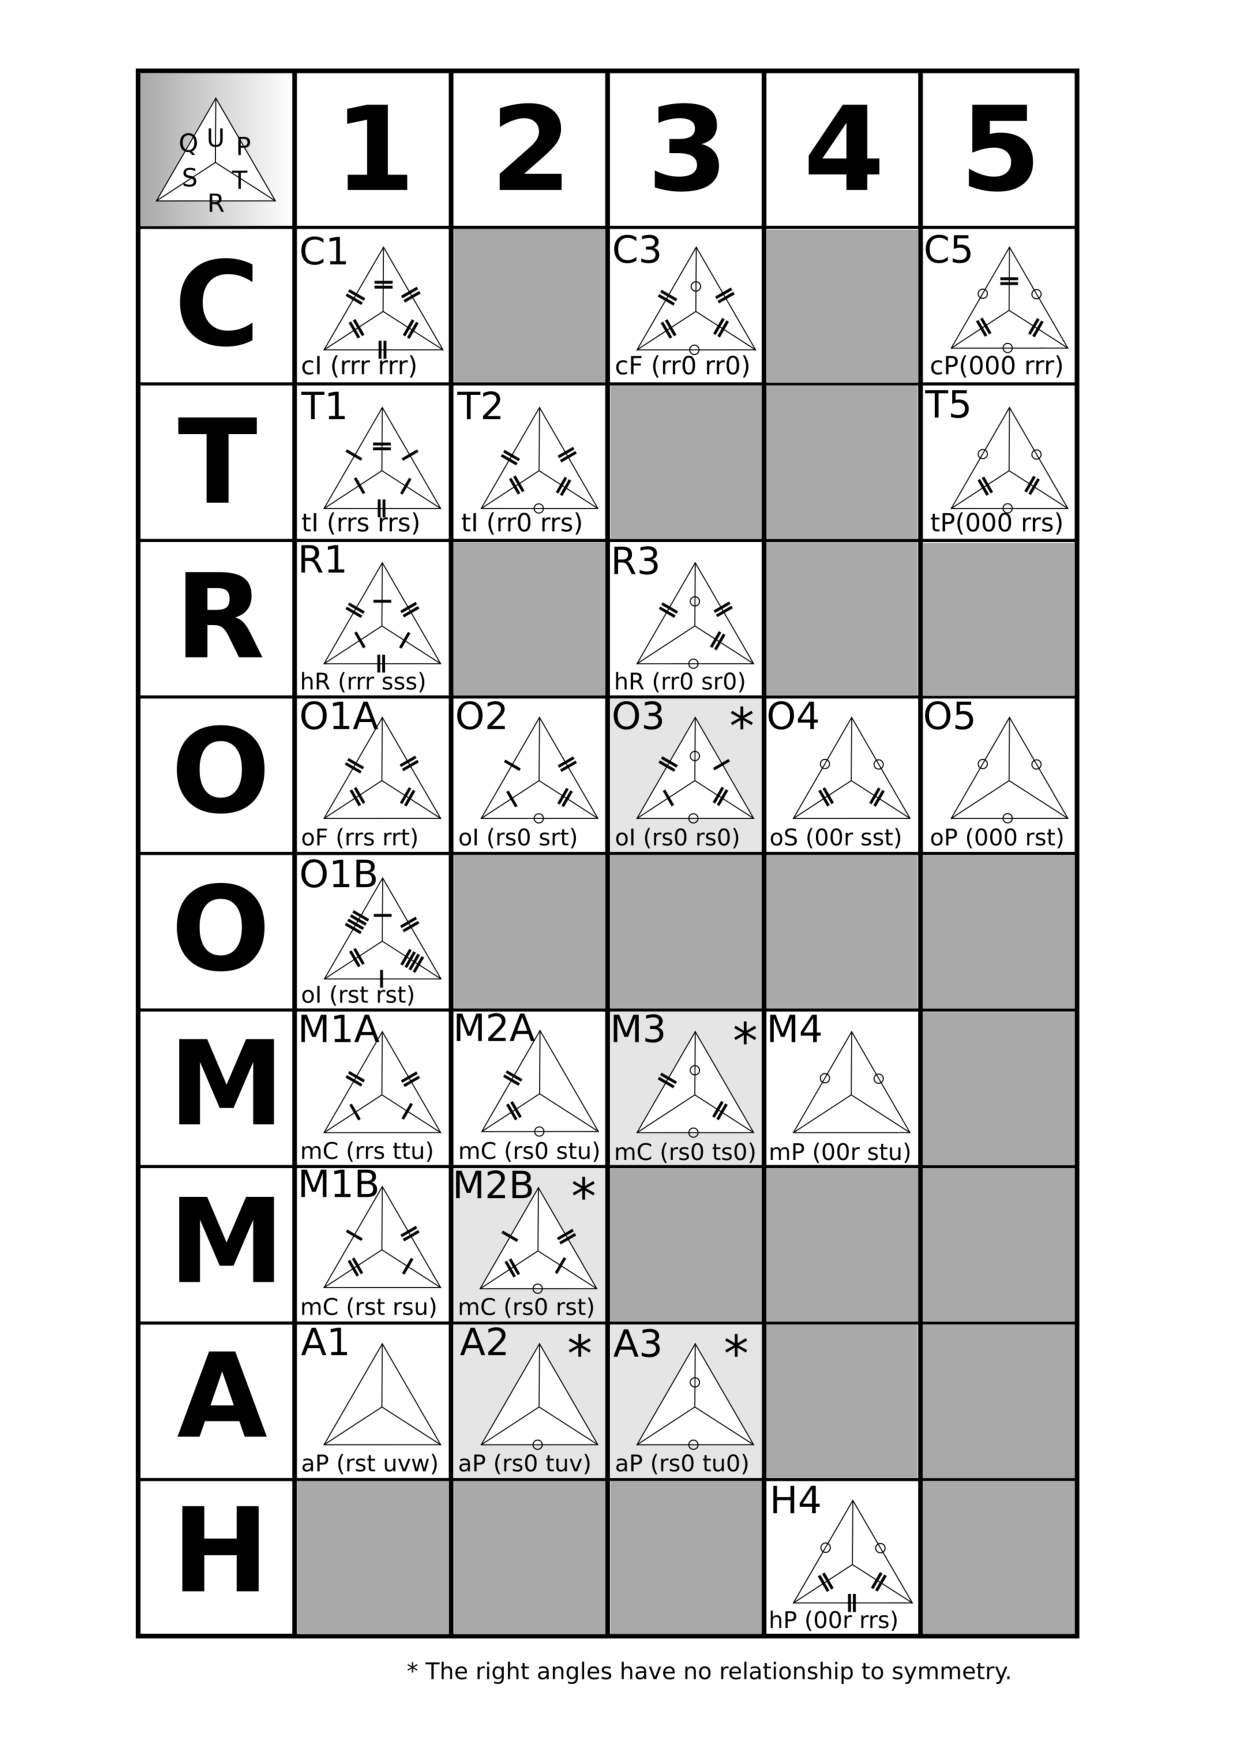
\includegraphics[width=0.85\textwidth]{DeloneTypesGrid_3}\\
		\label{s6table}		
	\end{table}

\begin{table}
	\caption{Roof/Niggli symbol, International Tables (IT) lattice character, Bravais lattice type, unsorted ${\mathbf{DC}^{\mathbf{7}}}$ subspace, boundary polytope.
		Note that the variables r, s and t are non-negative, and u, v and w may be
		positive, negative or zero as constrained below.}
	\begin{center}
		\begin{tabular}{|c|c|c|c|c|}
			\hline
			{\bf Roof/}     &{\bf IT}&{\bf Bravais}&{\bf Unsorted ${\mathbf{DC}^{\mathbf{7}}}$}&{\bf Bound-}\\
			{\bf Niggli}&{\bf Lattice}&{\bf Lattice}&{\bf Subspace}&{\bf ary}\\
			{\bf Symbol}&{\bf Char}&{\bf Type}&                             & {\bf Polytope} \\
			\hline
			44A&3&${\bf cP}$&$(r,r,r,2r,2r,2r,3r)$&$12345\!=\!12\hat{3}\!=\!12\hat{4}\!=\!12\hat{5}$\\
			\hline
			44C&1&$cF$&$(r,r,r,r,r,r,2r)$&12679ACD\\
			\hline
			44B&5&$cI$&$(r,r,r,4 r/3,4 r/3, 4 r/3,r)$&$\text{12F2}^{\prime} \text{F}^{\prime} = 1\hat{2}\hat{\text{F}}$\\
			\hline
			45A&11&${\bf tP}$&$(r,r,t,r+t,r+t,2r,2r+t)$&$1345 = 1\hat{3} = 1\hat{4} = 1\hat{5}$\\
			45B&21&${\bf tP}$&$(r,s,s,2s,r+s,r+s,r+2s$&$2345 = 2\hat{3} = 2\hat{4} = 2\hat{5}$\\
			\hline
			45D&6&$tI$&$(r,r,r,r-w/2,r-w/2,2r+w,r),$&\\
			&&&$-r \leq w \leq 0$&$\text{12FF}^{\prime} = 12\hat{\text{F}}$\\
			45D&7&$tI$&$[r,r,r,2*r+u,r-u/2,r-u/2,r],$&\\
			&&&$-r \leq u \leq 0$&$\text{12F2}^{\prime} = 1{\hat{2}}\text{F}$\\
			45C&15&$tI$&$(r,r,t,t,t,2r,t)$&158BF\\
			45E&18&$tI$&$(r,s,s,-r/2+2s,s,s,-r/2+2s)$&$\text{2ADA}^{\prime}  = 2{\hat{A}}\text{D}$\\
			\hline
			48A&12&${\bf hP}$&$(r,r,t,r+t,r+t,r,r+t])$&134E\\
			48B&22&${\bf hP}$&$(r,s,s,s,r+s,r+s,r+s)$&2458\\
			\hline
			49C&2&$hR$&$(r,r,r,2r-u,2r-u,2r-u,3r-u),$&\\
			&&&$0 < u \leq r$&$121^\prime 2^\prime = \hat{1}\hat{2}$\\
			49D&4&$hR$&$(r,r,r,2r+u,2r+u,2r+u,3r+3u),$&\\
			&&&$-r \leq u \leq 0$&$121^\prime 2^\prime = \hat{1}\hat{2}$\\
			49B&9&$hR$&$(r,r,t,t,t,r,r+t)$&1679ACD\\
			49E&24&$hR$&$(r,s,s,s+r/3,s+r/3,s+r/3,s)$&$2F2^\prime \text{F}^\prime = \hat{2}\hat{\text{F}}$\\
			\hline
			50C&32&${\bf oP}$&$(r,s,t,s+t,r+t,r+s,r+s+t)$&$345 = \hat{3} = \hat{4} = \hat{5}$\\
			\hline
			50D&13&$oC$&$(r,r,t,r+t,r+t,2r+w,2r+t+w),$&\\
			&&&$-r \leq w \leq 0$&134\\
			50E&23&$oC$&$(r,s,s,u+2*s,s+r,s+r,u+2*s+r),$&\\
			&&&$-s \leq u \leq 0$&245\\
			50A&36&$oC$&$(r,s,t,s+t,t,r+s,s+t)$&35B\\
			50B&38&$oC$&$(r,s,t,s+t,r+t,s,s+t)$&34E\\
			50F&40&$oC$&$[r,s,t,t,r+t,r+s,r+t)$&458\\
			\hline
			51A&16&$oF$&$(r,r,s,r+s+u,r+s+u,-2u,s),$&\\
			&&&$-r \leq u \leq 0$&$\text{1F1}^{\prime} = \hat{1}\text{F}$\\
			51B&26&$oF$&$(r,s,t,-r/2+s+t,t,s,-r/2+s+t)$&$\text{ADA}^{\prime}  = \hat{A}\text{D}$\\
			\hline
			52A&8&$oI$&$(r,r,r,2r+u,2r+v,-u-v,r),$&\\
			&&&$-r \leq u \leq 0, -r \leq v \leq 0$&12F\\
			52B&19&$oI$&$ (r,s,s,2s-u,s,s,-r+2s+u),$&\\
			&&&$0 < u \leq r $&\\
			&&&$ (r,s,s,2s-u,s,s,r+2s-u),$&\\
			&&&$r < u \leq s $&29C = 2AD\\
			52C&42&$oI$&$r,s,t,t,t,r+s,t$&58BF\\
			\hline
		\end{tabular}
	\end{center}
	\label{NiggliFormsI}
\end{table}%
	
		
	\begin{figure}
		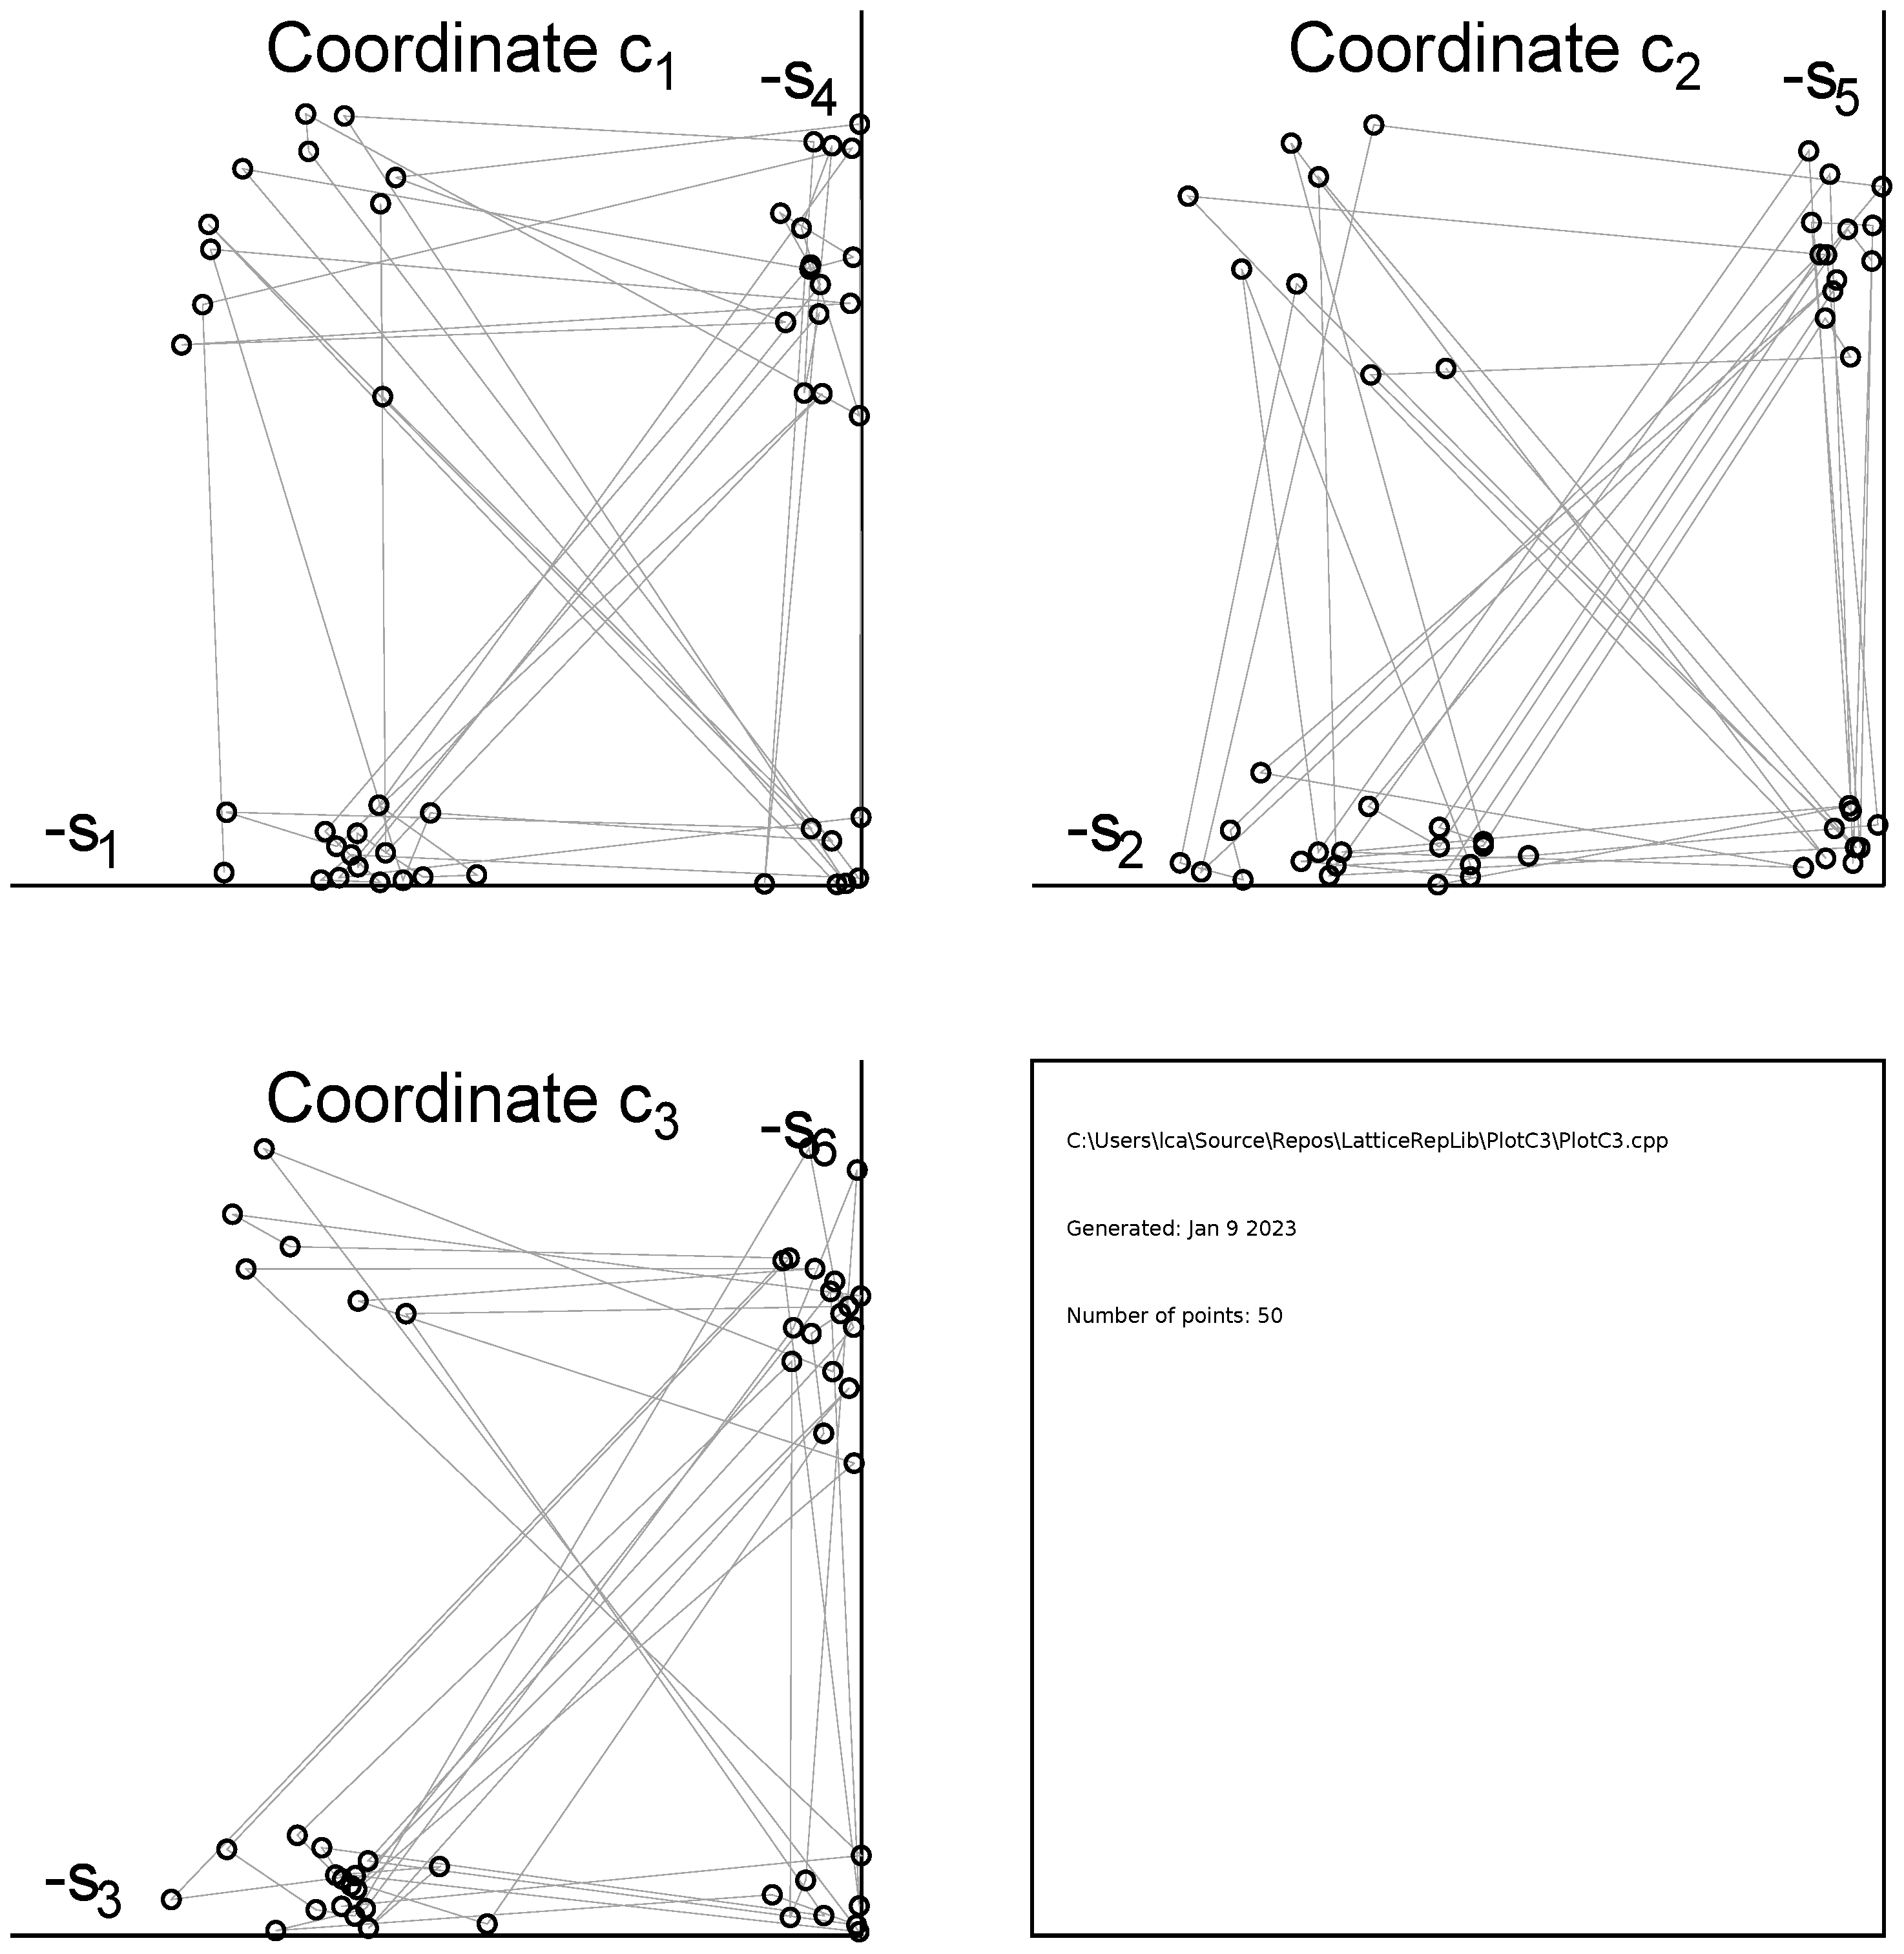
\includegraphics[width=\textwidth]{PlotC3}
		\label{plotc3}
		\caption{Output of PlotC3}
	\end{figure}
	
	\section{Availability of code}
	
	The $C^{++}$ ~code is available in github.com, in
	\url{https://github.com/duck10/LatticeRepLib.git}.
	
	\ack{\bf Acknowledgements}
	
	
	
	\ack{\bf Funding information}
	
	Funding for this research was provided in part by:  
	US Department of Energy Offices of Biological and 
	Environmental Research and of Basic Energy Sciences 
	(grant No. DE-AC02-98CH10886; grant No. E-SC0012704); 
	U.S. National Institutes of Health (grant No. P41RR012408; 
	grant No. P41GM103473; grant No. P41GM111244; 
	grant No. R01GM117126,
	grant No. 1R21GM129570); Dectris, Ltd.
	
	
		\bibliography{reduced}
		
		\bibliographystyle{iucr}
	
	
	
	%-------------------------------------------------------------------------
	% TABLES AND FIGURES SHOULD BE INSERTED AFTER THE MAIN BODY OF THE TEXT
	%-------------------------------------------------------------------------
	
	% Simple tables should use the tabular environment according to this
	% model
	
	% Postscript figures can be included with multiple figure blocks
	
	
	
\end{document}                    % DO NOT DELETE THIS LINE
%%%%%%%%%%%%%%%%%%%%%%%%%%%%%%%%%%%%%%%%%%%%%%%%%%%%%%%%%%%%%%%%%%%%%%%%%%%%%%
